\chapter{\label{ch:5-results}Results}


This section shows and discusses the results of our experiments based on the models and the datasets introduced in Chapter \ref{ch:4-methods}. It also describes the rationale behind deciding which experiments should be run.

\section{HEXEvent dataset} \label{sec:hexevent} %TODO> hexvent dataset section whether the other ones are not
To obtain a baseline, we evaluate the reimplemented and proposed model on the HEXEvent dataset as used in \cite{dsc} and introduced in \ref{sec:hexevent}. The results of these experiments are shown in Figure \ref{fig:hexevent_auc}. Generally all models perform extremely well with AUCs nearing 90\%. They also perform very similarly, making it hard to differentiate them based on the ROC curve. The Attn model seems to perform slightly better than the other models. 
There is a small (2\%) difference in the AUC values in the AUC values for the DSC model reported in \cite{dsc} (89.9 AUC) and the ones we observe (...). 
This is likely just a result of random statistical noise influenced by random seeds and differences between TensorFlow / Keras (their implementation) and PyTorch (our implementation).


\begin{figure}
	\centering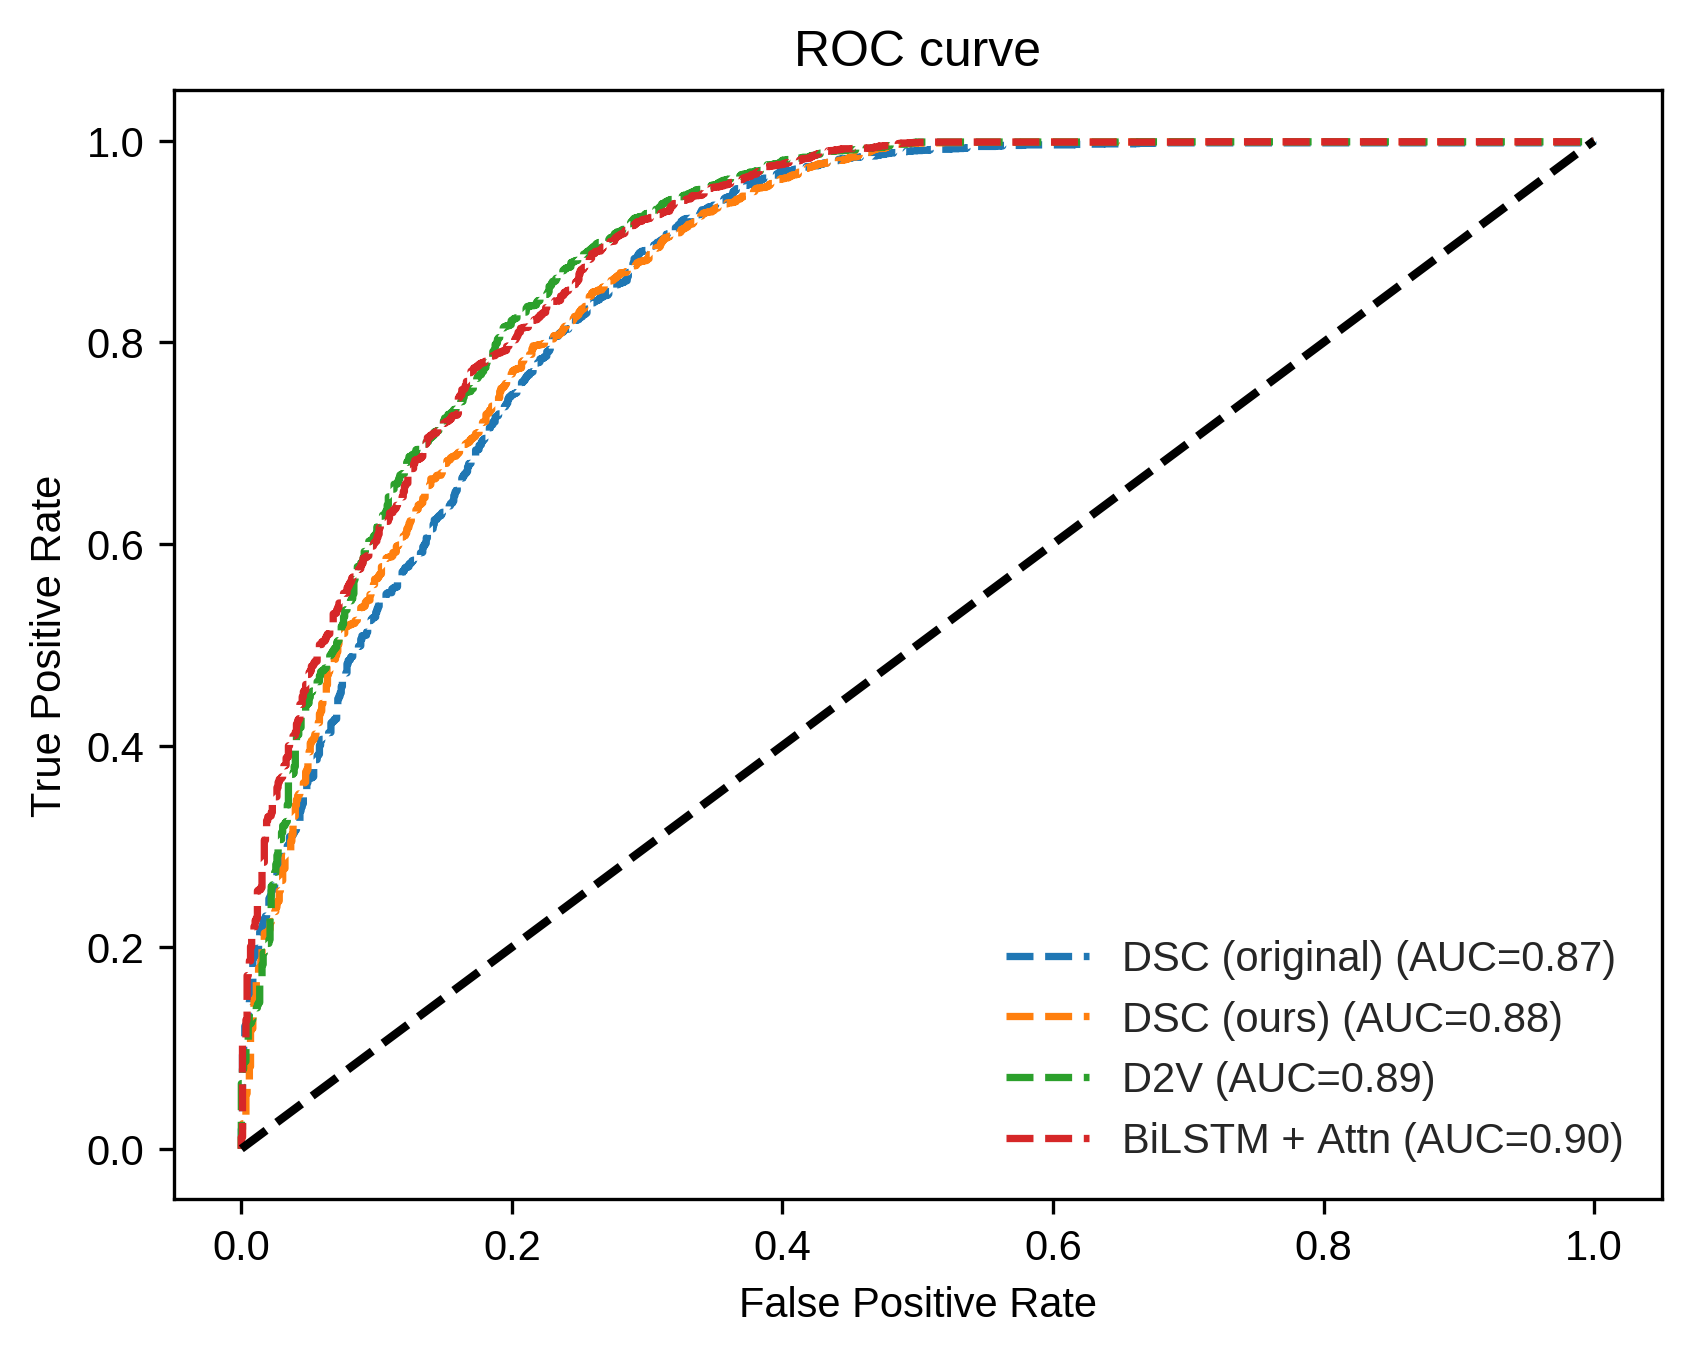
\includegraphics[width=0.7\textwidth]{../visualizations/hexevent_cross_model_roc_auc_comparison.png} 
	\caption[bla.]{Comparison of the ROC curves of the three main models (as well as the original implementation) on the HEXEvent dataset. The values of the original implementation were obtained by rerunning the training on the publicly available implementation. }
	\label{fig:hexevent_auc}
\end{figure}

main takeaway: all models perform extremely well \& very similarly



%To showcase the advantage of using the attention mechanism, we also included the BiLSTM-based model where only the last output is used for classification. This model performs significantly worse than the other ones.

% Observation: Performance heavily drops when no lengths feature is used


Reimplementation was done piece-wise, that is, first the sequence features were added as input, then the networks were trained to make sure that this was done correctly and then the length features were added. This lead to an interesting observation: model performance is significantly worse when no length features are given to the models. Quantitative results for this observation are given in table \ref{table:results_hexevent}. This observation is true across models and leads to a relative performance drop of ..... The information about the secondary structure obtained in the lengths seems to be necessary for the models to obtain good predictive power. 


\begin{table}[h!]
	\centering
	\begin{tabular}{| l | c | c | c| c} 
		\hline
		Model name & Only sequences & Sequences + lengths & Performance difference\\
		\hline
		DSC & 0.618 & 0.873 & 0.255\\
		D2V & 0.614 & 0.896 & 0.282\\
		BiLSTM + Attn & \textbf{0.636} & \textbf{0.904} & 0.268\\
		\hline
	\end{tabular}
	\caption{Performance of the main models on the HEXEvent dataset with and without length features given as AUC.  
	}
	\label{table:results_hexevent}
\end{table}


To further investigate, we also test three other models: MLP100, MLP20 and MLPLinear which respectively contain 100, 20 and 20 trainable parameters. They are simple MLPs with only one hidden layer which only take the length features as inputs. MLPLinear doesn't use a non-linear activation function after its hidden layer.

Surprisingly, the results in Figure \ref{fig:dsc_funeral} show that it is possible to replicate the results of \cite{dsc} with very simple models using two to three orders of magnitude fewer parameters. Model performance is improved by adding further parameters and breaks down when no non-linearities are used in the network. This indicates that there wasn't some mix-up during the data processing which would lead to even a linear model being able to predict alternative splicing, but that there is a non-trivial non-linear relationship which is being captured.
This leads to multiple possible explanations:
\begin{enumerate}
	\item there are confounders in the dataset learned by the model.
	\item either exon splicing is extremely well predictable based on the lengths of neighbouring introns and exons. This explanation, albeit unlikely already, can be disproven if this observation fails to replicate on other datasets.
	\item there are bugs (e.g. mixing of testing and validation data) in the reimplementation. However, this is unlikely given that we were able to replicate the original results of \cite{dsc}. To reduce complexity and further alleviate the likelihood of a bug leading to these observations, we extracted the complete code for replicating the results of the simple MLP models from \ref{fig:dsc_funeral} into a single file. 
\end{enumerate}
This indicates that 1) either exon splicing is extremely well predictable based on the lengths of neighbouring introns and exons or 2) there are confounders in the dataset learned by the model. 

These findings have strong implications. It calls into questions the meaningfulness of \cite{dsc}'s results, showing the competitiveness of their model. These findings likely also warrant a critical investigation of any other conclusions drawn from papers based on the HEXEvent database. At the time of writing, the HEXEvent paper is cited 34 times. While most of these citations are just in passing, there are also multiple papers which use a HEXEvent-derived dataset for the training of Machine Learning models \cite{buschhertel} 

Recognition of alternatively spliced cassette exons based on a hybrid model -- confirmed
A classification of alternatively spliced cassette exons using AdaBoost-based algorithm
G2P: Using machine learning to understand and predict genes causing rare neurological disorders --- definitely in some capacity
Exon size and sequence conservation improves identification of splice-altering nucleotides

Bugs in the replication  are unlikely given that the same implementation was also able to reproduce [dsc papers]'s original results.


a) is extremely unlikely given that research into splicing has been ongoing for 50 years. a) can be disproven if this result fails to replicate on other datasets.
b) is substantially more likely, especially giving the discussions of biases in EST-based data. The biases inherent in EST-based data could be captured by the exon and intron structure and the model is learning to make its prediction based on this bias. b) can be shown if this result fails to replicate on other datasets. 


We showed that the EST-based HEXEvent dataset is likely too flawed to serve as a basis for our methods. Thus, we try to construct an alternative dataset.



\begin{figure}
	\centering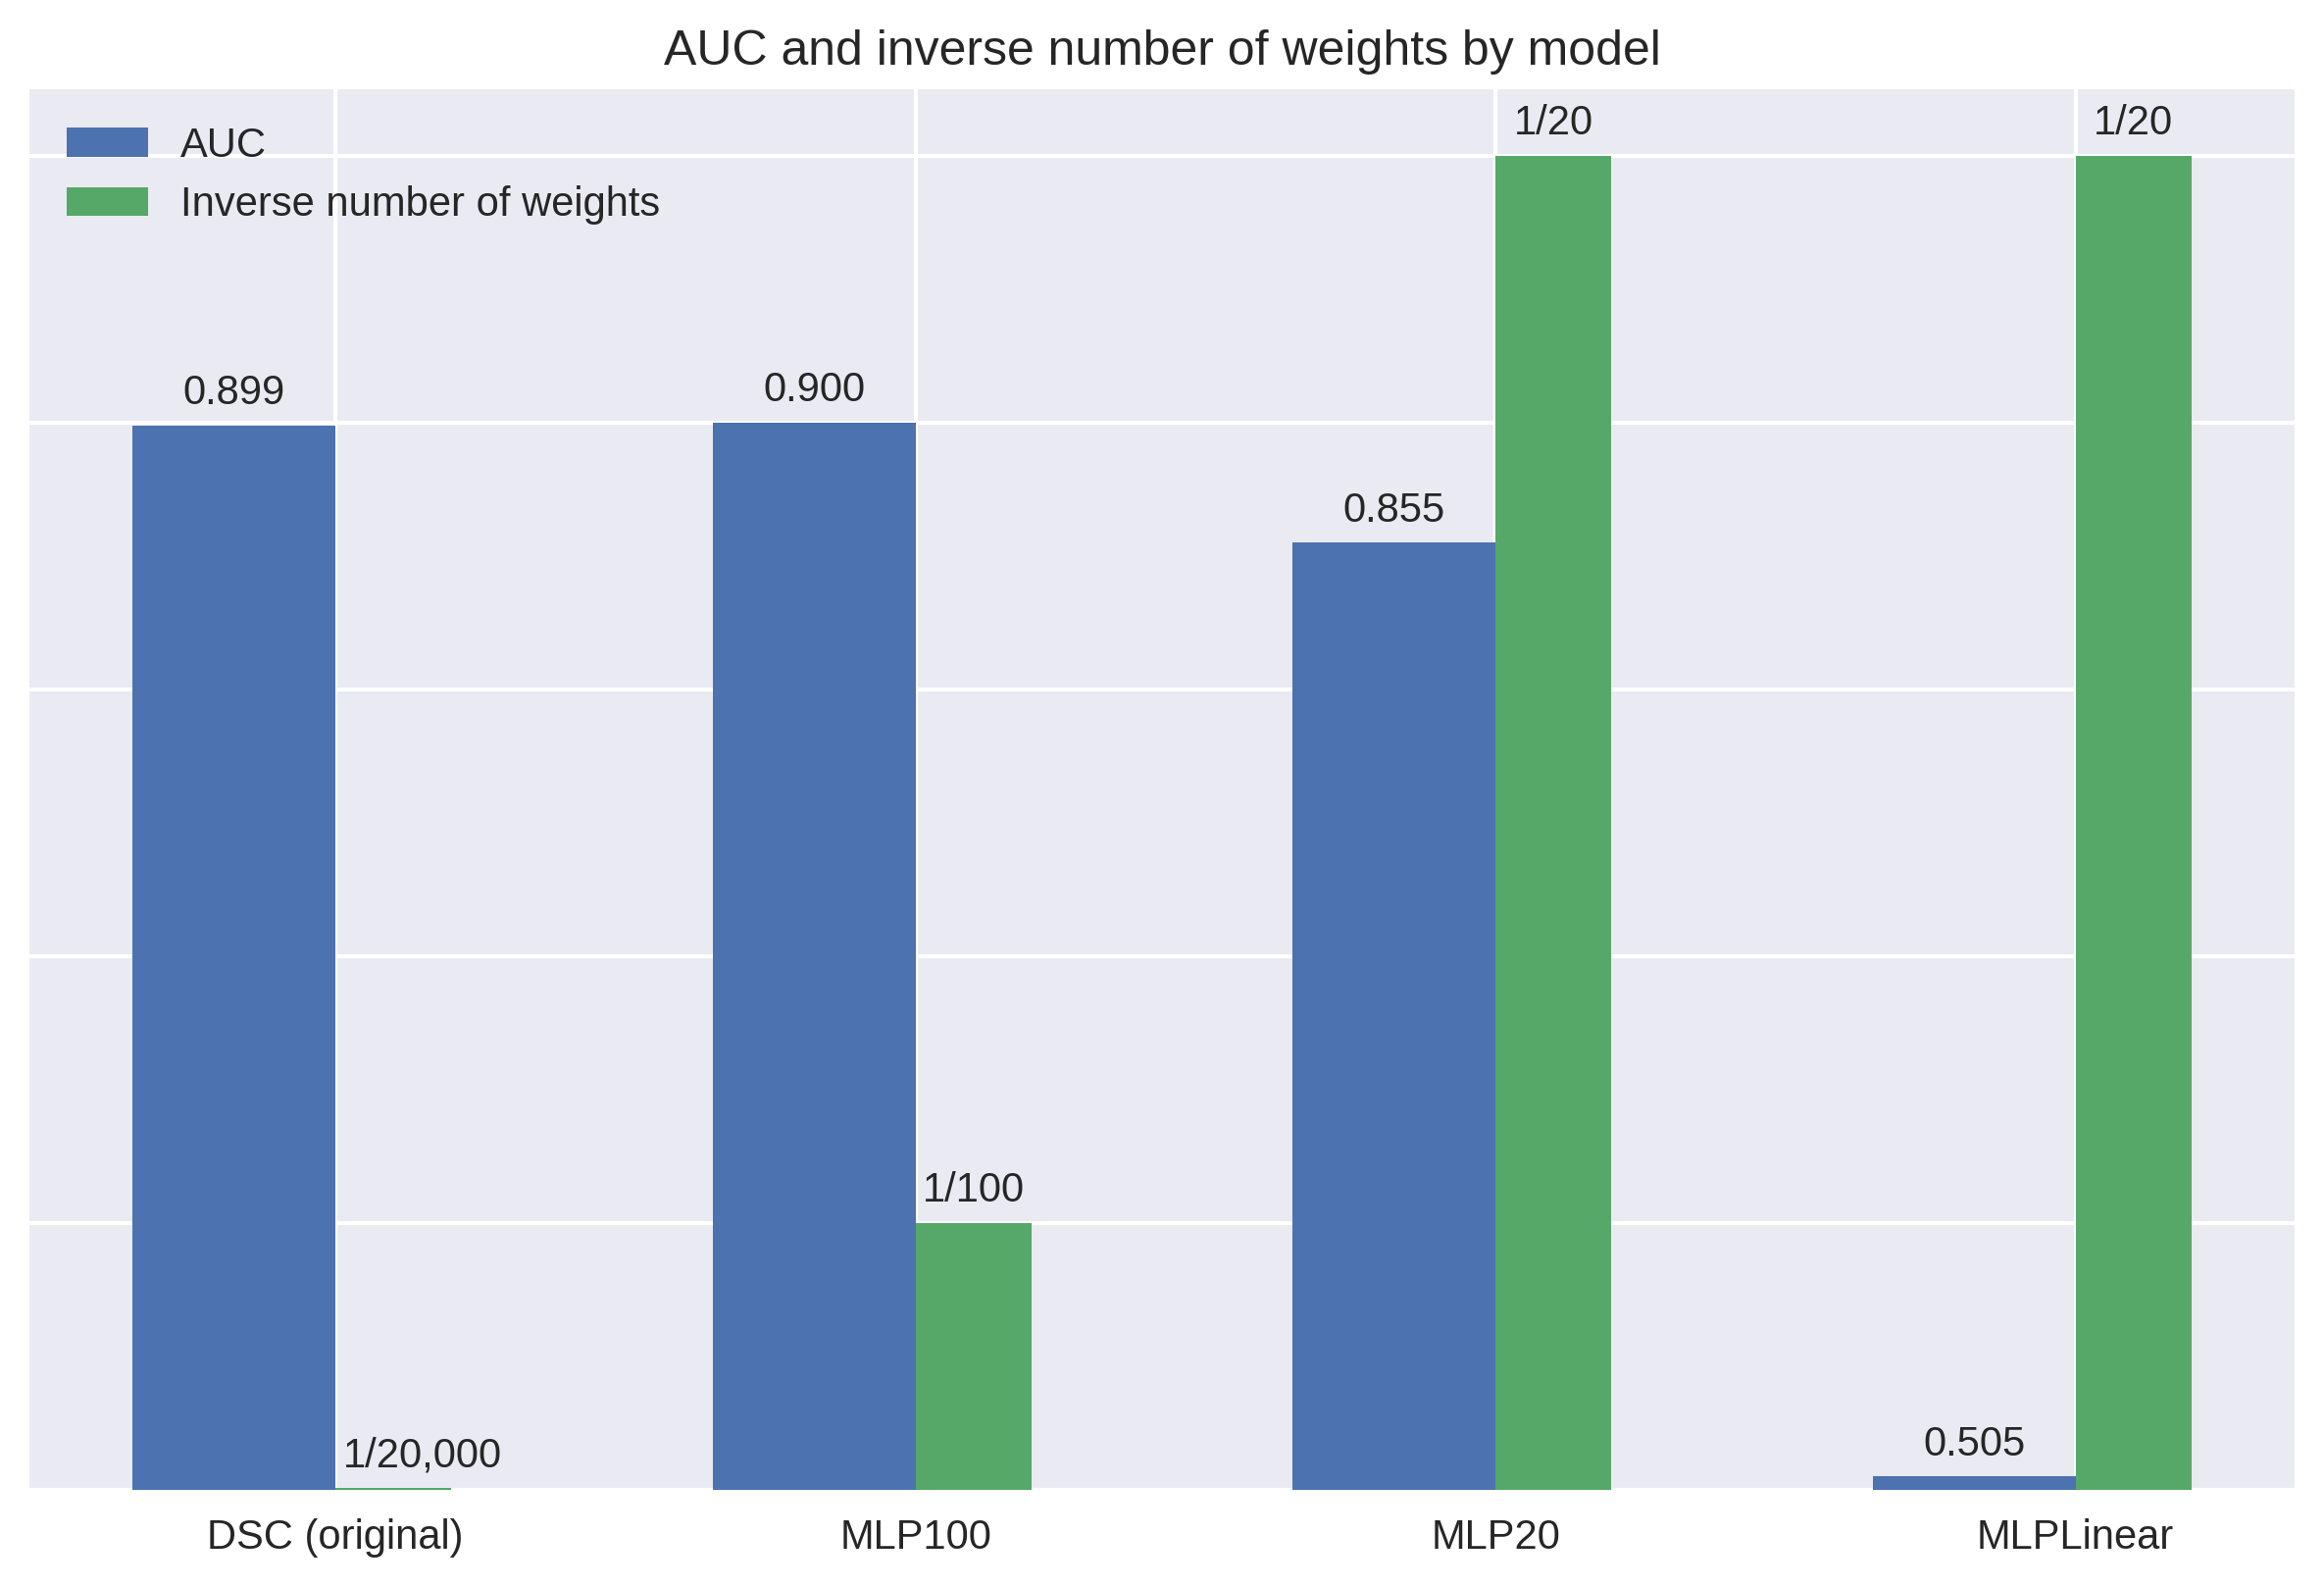
\includegraphics[width=0.7\textwidth]{../visualizations/dsc_funeral_barchart.png} 
	\caption[bla.]{Stress testing the HEXEvent dataset used in \cite{dsc}. The graph shows the performance as well as the inverse of the respective model sizes used.}
	\label{fig:dsc_funeral}
\end{figure}

TODO: tSNE of MLP embeddings?


\section{GTEx-based datasets} \label{sec:gtex}

\section{HipSci-based dataset} \label{sec:hipsci} 
\subsection{SUPPA with neuron tissue induced iPSCs} \label{subsec:hipsci_suppa}

\begin{figure}
	\centering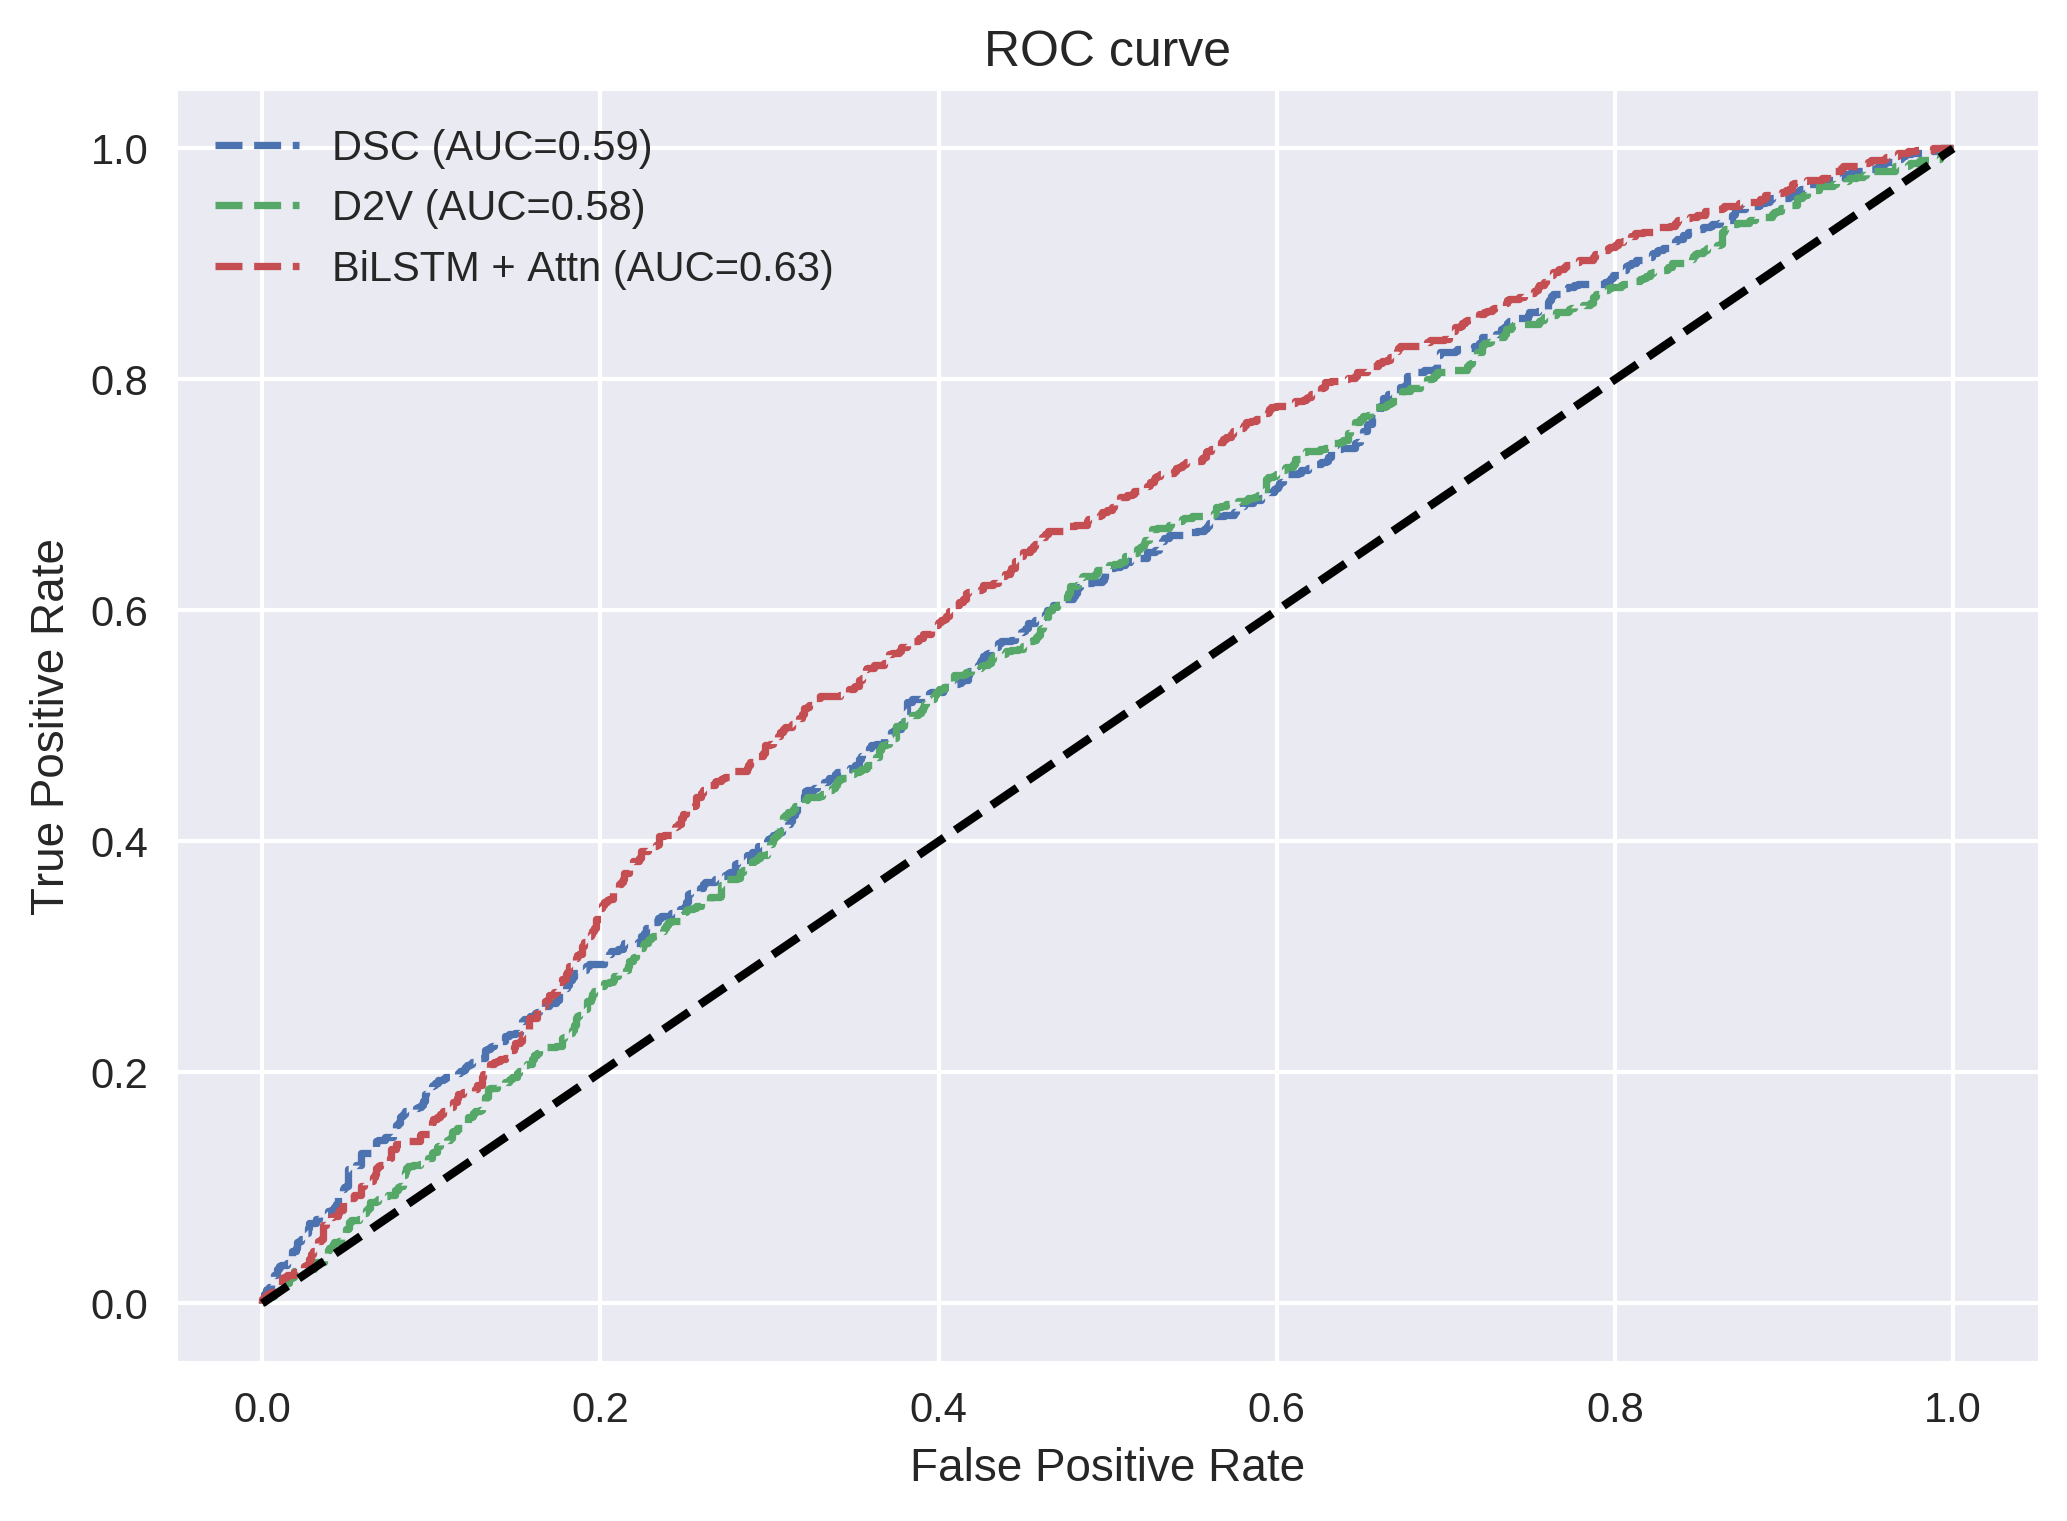
\includegraphics[width=0.7\textwidth]{../visualizations/suppa_cross_model_roc_auc_comparison.png} 
	\caption[bla.]{Comparison of the ROC curves of the three main models on the HipSci dataset derived by using SUPPA. }
	\label{fig:suppa_auc}
\end{figure}

Takeaways:
\begin{enumerate}
	\item All models perform similarly, BiLSTM + Attn tends to perform best
	\item All models perform very poorly perhaps a dataset issue (due to HIPSCI SUPPA being coarse-grained)
\end{enumerate}

\subsection{MAJIQ with neuron tissue induced iPSCs} \label{sec:hipsci_majiq}
